% ==============================================================================
% Chapter 7: Risk Management, 24-Month Roadmap, Budget & Success KPIs
% ==============================================================================
\chapter{ניהול סיכונים, תוכנית עבודה הנדסית, תקציב ומדדי הצלחה}
\label{ch:roadmap}

\section{ניהול סיכונים אסטרטגיים, טכנולוגיים וחוקתיים}
הטמעת תשתית לאומית להגנת התודעה כרוכה בסיכונים הדורשים מענה הנדסי ומוסדי מראש. איומים אלה אינם נובעים רק מכשלי תוכנה או חומרה, אלא גם מתוקפים אדברסריים המנסים להטעות את המערכת עצמה ("התקפות יריב"), ומתרחישים של שחיקת אמון הציבור. טבלה~\ref{tab:risk_matrix} מסכמת את מפת שבעת הסיכונים המרכזיים ואת מערך הבלימה שתוכנן עבורם.

{\renewcommand{\arraystretch}{1.35}
\begin{table}[htbp]
\centering
\caption{מטריצת ניהול סיכונים של פרויקט CivicShield AI ודרכי מיטיגציה}
\label{tab:risk_matrix}
\begin{tabularx}{\textwidth}{|p{2.7cm}|p{1.6cm}|p{1.6cm}|X|p{2.0cm}|}
\hline
\textbf{\textcolor{CivicNavy}{תיאור הסיכון}} & \textbf{\textcolor{CivicNavy}{סבירות}} & \textbf{\textcolor{CivicNavy}{חומרה}} & \textbf{\textcolor{CivicNavy}{מנגנון בלימה ומיטיגציה הנדסית}} & \textbf{\textcolor{CivicNavy}{סיכון שיורי}} \\ \hline
התקפת \en{Prompt Injection} בטקסט רשת & גבוהה & קריטית & אימות תחבירי קשיח (\en{JSON Pydantic}), הפרדת הוראות מדאטה ובידוד סוכנים בארגז חול. & נמוך \\ \hline
הטיה מפלגתית בסיווג מסגור & בינונית & קריטית & מבדק שוויון דו-מפלגתי שבועי (\en{NFR-05}), פיקוח חוקתי וגילוי נאות בקוד פתוח. & נמוך \\ \hline
התחמקות מתואמת (\en{Adversarial Evasion}) & גבוהה & גבוהה & איחוד 4 מודאליות בייסיאני (\en{Audio/Video/C2PA/Graph}); התוקף נדרש לזייף את כולן יחד. & בינוני-נמוך \\ \hline
צוואר בקבוק בזמן סגירת הקלפיות & בינונית & גבוהה & קנה מידה דינמי ל-\en{34 GPU Pools} ושרידות \en{Multi-AZ} תחת מודל \en{M/M/c}. & נמוך \\ \hline
דליפת מידע מזהה של אזרחים & נמוכה & קריטית & מחיקת \en{PII} בכניסה, \en{$\epsilon \le 1.2$} פרטיות דיפרנציאלית ומחיקה אוטומטית כל 30 יום. & מזערי \\ \hline
ניצול לרעה על ידי הרשות המבצעת & נמוכה & קריטית & מנגנון חתימה משולשת (\en{3-of-3 Ed25519 Quorum}) כולל זכות וטו שיפוטית ואופוזיציונית. & מזערי \\ \hline
עייפות תודעתית מאזהרות (\en{Alert Fatigue}) & בינונית & בינונית & תזמון אזהרות ממוקד רק בחציית סף התפרצות \en{$R_0 > 1.5$} והגבלת תדירות לציבור. & נמוך \\ \hline
\end{tabularx}
\end{table}}

\section{תוכנית עבודה הנדסית רב-שלבית ל-24 חודשים (Roadmap)}
הקמת מערכת \en{CivicShield AI} מתוכננת בפריסה מדורגת על פני ארבעה שלבים בני חצי שנה כל אחד (סה"כ 24 חודשים), כך שכבר בתום השנה הראשונה ניתן יהיה להפעיל תשתית צללים פאסיבית (\en{Shadow Mode}) לצורכי כיול וביקורת טרם העלייה המבצעית המלאה.
\begin{itemize}
    \item \textbf{שלב א' (חודשים 1–6) — תשתית קליטה, פרטיות ויומן ביקורת:} הקמת מאגרי \en{Kafka/Flink} בארכיטקטורת \en{Multi-AZ}, הטמעת מסנן \en{$\epsilon$-DP}, בניית ארגזי החול ומערך הביקורת ה-\en{Merkle}, וקליטת מדגם היסטורי לאימון ב-3 שפות.
    \item \textbf{שלב ב' (חודשים 7–12) — ועדת הסוכנים ומנועי הפורנזיקה:} פיתוח ואימון של סוכני הרשת (\en{CIB}), מסגור אנטמן בעברית ובערבית, גלאי ה-\en{Deepfake} הבייסיאני ומנוע הסימולציות \en{SIRI} ו-\en{Hegselmann-Krause} ב-\en{Python}.
    \item \textbf{שלב ג' (חודשים 13–18) — שער חוקתי, משחקי מלחמה ואיזון פוליטי:} התקנת מנוע המדיניות \en{OPA/Rego}, הטמעת מערכת החתימה הקריפטוגרפית המשולשת, וביצוע סדרת תרגילי צוות אדום (\en{Red-Team Wargames}) עם אוניברסיטאות ומשפטנים.
    \item \textbf{שלב ד' (חודשים 19–24) — הקשחה, אלסטיות והפעלה לאומית:} מבחני עומס של \en{12,000 EPS} עם \en{34 GPU Pools}, חניכת פורטל השקיפות הפומבי וממשקי התקשורת, וקבלת תו כשירות סופי מוועדת הבחירות.
\end{itemize}

איור~\ref{fig:roadmap_gantt} מציג את תרשים הגאנט ההנדסי המלא על ציר הזמן של 24 החודשים.

\begin{figure}[htbp]
\begin{tikzhebrew}
\begin{tikzpicture}[scale=1.0]
    % Frame & Header Timeline (0 to 9.6 cm -> each 0.4 cm = 1 month -> 24 months = 9.6 cm)
    % Labels on left from -5.4 to -0.2 cm -> total width 15.0 cm
    \fill[CivicNavy] (-6.0, 4.7) rectangle (9.8, 5.45);
    \node[text=white, font=\bfseries\small] at (-3.1, 5.07) {\he{שלב / תת-תוכנית הנדסית}};
    \node[text=white, font=\bfseries\small] at (4.8, 5.07) {\he{לוח זמנים להקמה (חודשים 1 עד 24)}};

    % Vertical Quarter Grid Lines & Month Markers
    \foreach \m/\lbl in {0/M1, 2.4/M6, 4.8/M12, 7.2/M18, 9.6/M24} {
        \draw[CivicSlate!45!white, dashed] (\m, 0.2) -- (\m, 4.65);
    }
    \node[font=\scriptsize\bfseries, text=CivicNavy] at (0, 4.38) {M1};
    \node[font=\scriptsize\bfseries, text=CivicNavy] at (2.4, 4.38) {M6};
    \node[font=\scriptsize\bfseries, text=CivicNavy] at (4.8, 4.38) {M12};
    \node[font=\scriptsize\bfseries, text=CivicNavy] at (7.2, 4.38) {M18};
    \node[font=\scriptsize\bfseries, text=CivicNavy] at (9.35, 4.38) {M24};

    % Row backgrounds
    \fill[CivicGrayBg] (-6.0, 3.35) rectangle (9.8, 4.10);
    \fill[white] (-6.0, 2.50) rectangle (9.8, 3.25);
    \fill[CivicGrayBg] (-6.0, 1.65) rectangle (9.8, 2.40);
    \fill[white] (-6.0, 0.80) rectangle (9.8, 1.55);
    \fill[CivicGoldBg] (-6.0, 0.05) rectangle (9.8, 0.70);

    % Task Labels (Hebrew wrapped safely)
    \node[anchor=east, font=\footnotesize\bfseries, text=CivicNavy] at (-0.25, 3.72) {\he{שלב א': תשתית, \en{OSINT} ו-\en{$\epsilon$-DP}}};
    \node[anchor=east, font=\footnotesize\bfseries, text=CivicNavy] at (-0.25, 2.87) {\he{שלב ב': סוכנים, מסגור ו-\en{Deepfake}}};
    \node[anchor=east, font=\footnotesize\bfseries, text=CivicNavy] at (-0.25, 2.02) {\he{שלב ג': שער חוקתי ומשחקי \en{RedTeam}}};
    \node[anchor=east, font=\footnotesize\bfseries, text=CivicNavy] at (-0.25, 1.17) {\he{שלב ד': מבחני עומס \en{12k} והפעלה}};
    \node[anchor=east, font=\footnotesize\bfseries, text=CivicGold!80!black] at (-0.25, 0.37) {\he{מבצעיות שוטפת ומבחני שוויון}};

    % Gantt Bars (each month = 0.4 cm)
    % Phase 1: M1-M6 (0 to 2.4)
    \fill[CivicNavy, rounded corners=2pt] (0.05, 3.50) rectangle (2.40, 3.95);
    \node[text=white, font=\tiny\bfseries] at (1.22, 3.72) {\en{M1-M6}};

    % Phase 2: M6-M13 (2.0 to 5.2)
    \fill[CivicBlue, rounded corners=2pt] (2.00, 2.65) rectangle (5.20, 3.10);
    \node[text=white, font=\tiny\bfseries] at (3.60, 2.87) {\en{M6-M13}};

    % Phase 3: M12-M19 (4.4 to 7.6)
    \fill[CivicTeal, rounded corners=2pt] (4.40, 1.80) rectangle (7.60, 2.25);
    \node[text=white, font=\tiny\bfseries] at (6.00, 2.02) {\en{M12-M19}};

    % Phase 4: M18-M24 (6.8 to 9.6)
    \fill[CivicEmerald, rounded corners=2pt] (6.80, 0.95) rectangle (9.60, 1.40);
    \node[text=white, font=\tiny\bfseries] at (8.20, 1.17) {\en{M18-M24}};

    % Continuous Governance Track: M7-M24
    \fill[CivicGold, rounded corners=2pt] (2.40, 0.20) rectangle (9.60, 0.55);
    \node[text=white, font=\tiny\bfseries] at (6.00, 0.37) {\he{ביקורת שופטים ומבדק הטיה דו-שבועי}};

    % Milestones Diamonds
    \node[diamond, fill=CivicRed, draw=white, inner sep=2.2pt] at (5.20, 2.87) {};
    \node[diamond, fill=CivicRed, draw=white, inner sep=2.2pt] at (7.60, 2.02) {};
    \node[diamond, fill=CivicRed, draw=white, inner sep=2.2pt] at (9.60, 1.17) {};

    \draw[CivicNavy, line width=0.9pt] (-6.0, 0.05) rectangle (9.8, 5.45);
\end{tikzpicture}
\end{tikzhebrew}
\caption{מפת דרכים הנדסית ל-24 חודשים (Gantt) להקמת והקשחת מערכת CivicShield AI}
\label{fig:roadmap_gantt}
\end{figure}

\section{תקציב חמש-שנתי, כלכלת טוקנים ותשואה מוסדית (ROI)}
בניית מערכת בינה מלאכותית לאומית מתמודדת לעיתים עם הפתעות תקציביות בשל עלויות עיבוד שוטפות (\en{Tokenomics \& GPU Cluster OPEX}). בזכות תכנון הארכיטקטורה המדורגת (שכבה 2 מפעילה סינון מהיר ומעבירה לשכבה 3 רק \en{6\%} לסוכן טריאז' ו-\en{0.8\%} לוועדת ה-\en{ReAct} המלאה), עלות התפעול השוטפת נשמרת מאוזנת ויציבה לאורך 5 שנים.

טבלה~\ref{tab:budget_5yr} מפרטת את אומדן התקציב החמש-שנתי במיליוני ש"ח, ואיור~\ref{fig:budget_roi} משווה את עלות הבעלות הכוללת (\en{Cumulative TCO = 68.7M NIS}) אל מול הערך החסוך ממניעת שיבוש בחירות, הונאות מוסדיות ושחיקת אמון (\en{Cumulative Value = 145.0M NIS}), עם נקודת איזון כלכלי (\en{Break-Even}) בשנה \en{2.2}.

{\renewcommand{\arraystretch}{1.35}
\begin{table}[htbp]
\centering
\caption{פירוט תקציב חמש-שנתי (CAPEX / OPEX) וערך חוסן מוסדי (במיליוני ש"ח)}
\label{tab:budget_5yr}
\begin{tabularx}{\textwidth}{|p{2.3cm}|c|c|c|c|X|}
\hline
\textbf{\textcolor{CivicNavy}{שנת תוכנית}} & \textbf{\textcolor{CivicNavy}{CAPEX}} & \textbf{\textcolor{CivicNavy}{OPEX}} & \textbf{\textcolor{CivicNavy}{סה"כ עלות}} & \textbf{\textcolor{CivicNavy}{ערך חוסן}} & \textbf{\textcolor{CivicNavy}{רכיב הוצאה מרכזי בתקציב}} \\ \hline
שנה 1 (הקמה) & \en{14.5} & \en{6.5} & \en{21.0} & \en{8.0} & חומרת ליבה, צינור \en{OSINT} ומודלי בסיס \\ \hline
שנה 2 (שילוב) & \en{4.0} & \en{8.2} & \en{12.2} & \en{22.0} & רשת סוכנים, צוות אדום וכלי חיסון \\ \hline
שנה 3 (בחירות) & \en{2.5} & \en{8.8} & \en{11.3} & \en{31.0} & שיא עומס אלסטי (\en{34 Pools}) ובלימת משברים \\ \hline
שנה 4 (הרחבה) & \en{3.0} & \en{9.4} & \en{12.4} & \en{38.0} & תמיכה בבחירות מקומיות והנגשת \en{XAI} \\ \hline
שנה 5 (תחזוקה) & \en{2.0} & \en{9.8} & \en{11.8} & \en{46.0} & רענון מודלים אל מול טכנולוגיות זיוף עתידיות \\ \hline
\textbf{\textcolor{CivicNavy}{סה"כ 5 שנים}} & \textbf{\en{26.0}} & \textbf{\en{42.7}} & \textbf{\en{68.7}} & \textbf{\en{145.0}} & \textbf{נקודת איזון (\en{ROI Break-Even}) בשנה \en{2.2}} \\ \hline
\end{tabularx}
\end{table}}

\begin{figure}[htbp]
\centering
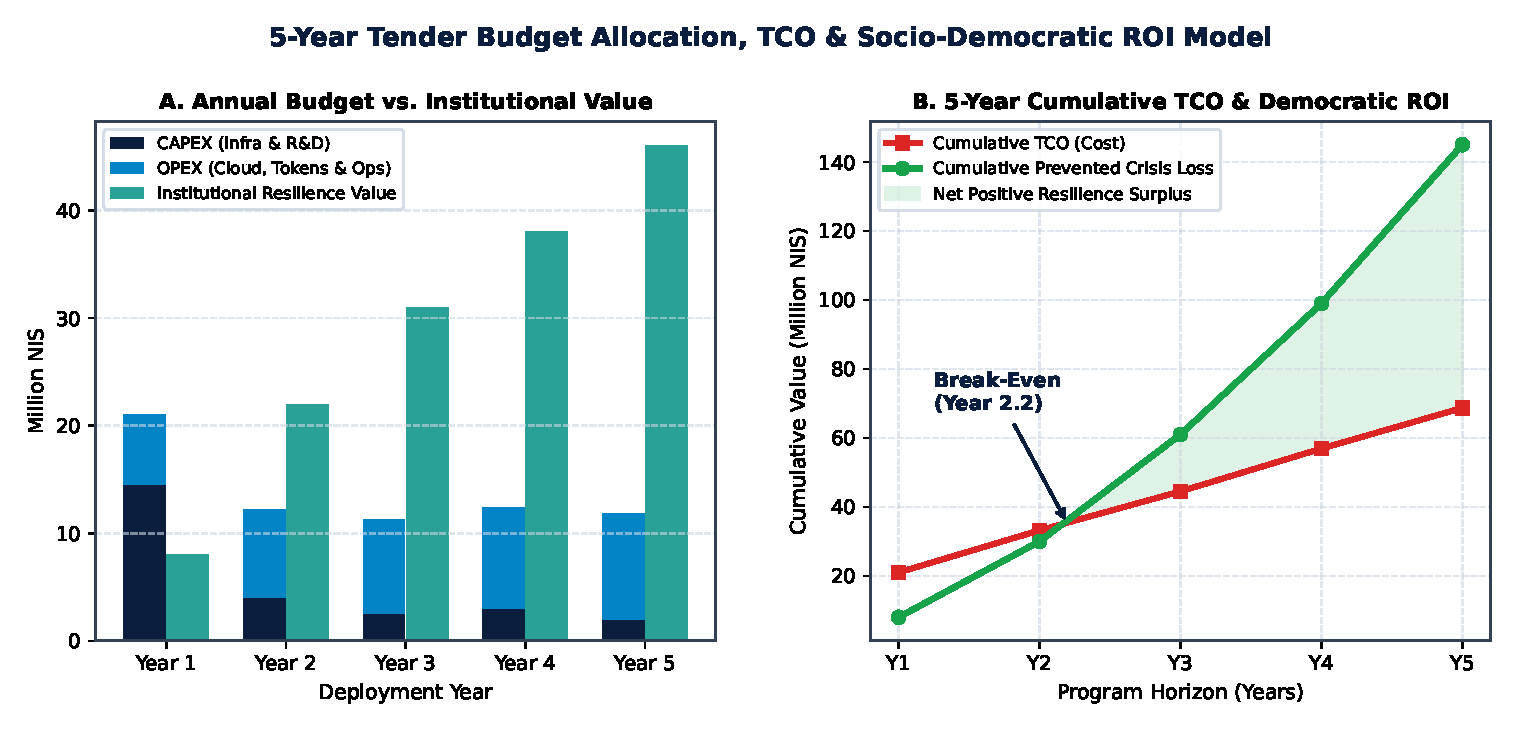
\includegraphics[width=0.95\textwidth]{figures/fig6_budget_roi_projection.pdf}
\caption{תחזית תקציב חמש-שנתית (CAPEX/OPEX), עלות בעלות כוללת (TCO) והחזר השקעה מוסדי}
\label{fig:budget_roi}
\end{figure}

\section{מדדי הצלחה מחייבים ורמת שירות (SLA / KPI Framework)}
קבלת הפרויקט מהקבלן המבצע ומסירתו לידי ועדת הבחירות המרכזית ומערך הסייבר מותנות בעמידה מדידה בחמישה מדדי ליבה מרכזיים (טבלה~\ref{tab:kpi_sla}).

{\renewcommand{\arraystretch}{1.35}
\begin{table}[htbp]
\centering
\caption{מסגרת מדדי הצלחה ורמות שירות (KPIs \& SLAs) לתנאי מסירת הפרויקט}
\label{tab:kpi_sla}
\begin{tabularx}{\textwidth}{|p{3.0cm}|p{2.7cm}|p{2.9cm}|X|}
\hline
\textbf{\textcolor{CivicNavy}{שם המדד (\en{KPI})}} & \textbf{\textcolor{CivicNavy}{ערך סף מחייב}} & \textbf{\textcolor{CivicNavy}{תדירות מדידה}} & \textbf{\textcolor{CivicNavy}{שיטת אימות אובייקטיבית}} \\ \hline
זמן תגובה בקצה (\en{E2E Latency}) & \en{$\le 250\,\text{ms}$} & רציף (\en{P95}) & מדידת שיהוי ב-\en{Load Test} מול \en{12,000 EPS}. \\ \hline
זמן גילוי והפקת \en{Prebunking} & \en{$\le 30\,\text{דקות}$} & לכל אירוע קריטי & חותמת זמן מרגע זריעה בטלגרם ועד הכנת תבנית חיסון. \\ \hline
דיוק זיהוי \en{Deepfake} משולב & \en{$\text{Precision} \ge 90\%$} & חודשי + סקר תקופתי & ביקורת עיוורת על מאגר זיופים מבוקר בתיאום אקדמי. \\ \hline
פער שוויון פוליטי (\en{Fairness}) & \en{$\Delta \text{FPR} < 1.5\%$} & דו-שבועי & הרצת סימולציית ביקורת סימטרית על כלל המחנות. \\ \hline
אפס מקרי אכיפה ללא קוורום & \en{0 חריגות} & רציף (שער קריפטו) & אימות שלמות יומן ה-\en{Merkle} ומפתחות ה-\en{Ed25519}. \\ \hline
\end{tabularx}
\end{table}}
